\section{Variations}
\label{sec:variations}
Many variations of the basic MCTS approach have been proposed by the research community. This section presents some notable developments in recent years. Section \ref{ss:mab} considers new results with respect to Multi-Armed Bandits and methods of determining upper confidence bounds. Section \ref{ss:heuristics} describes heuristics to improve general MCTS algorithms while Sections \ref{ss:real_time} and \ref{ss:multi_agents} lay out more narrow approaches to apply MCTS in certain domains, namely real-time scenarios and situations where multiple instances of the search algorithm are executed in agents that need to cooperate. Finally, Section \ref{ss:evo_alg} presents a novel way of using the framework of evolutionary algorithms in conjunction with MCTS.
\subsection{MAB and UCB-Tuning}
\label{ss:mab}
\paragraph{Fixed Budgets}
The \textit{fixed budgets} setting (as opposed to \textit{fixed confidence} \cite{jamieson2014best}) describes the constraint of a MAB-problem that the best possible arm must be identified using no more than $m$ \enquote{pulls}.
Karnin et al. \cite{karnin2013almost} provide (what they call) an almost optimal exploration algorithm in this setting called \textit{Sequential Halving} given in Algorithm \ref{alg:sequential_halving}. Each arm of the MAB problem is associated with a random variable yielding values in the interval $[0,1]$. W.l.o.g the $k$ different arms are ordered according to their expected value $p_i \in [0,1]$ at every decision epoch $t$: $p_1, \geq p_2 \geq \ldots \geq p_k$. $\Delta_i \coloneqq p_1 - p_i$ denotes the suboptimality gap of arm $i$. Consequently, $\Delta_2$ is the smallest of all these gaps. It can be shown that for the required budget $T$ for identifying the best arm with a probability of at least $(1-\delta)$ we have $T \in \Omega(H \log (\frac{1}{\delta}))$ where $H \coloneqq \sum_{i=2}^{k} \frac{1}{\Delta_i^2}$. $H$ is a measure of the complexity of the problem. Another related measure is given via: $H_2 \coloneqq \max_{i \neq 1} \frac{i}{\Delta_i^2}$. With these considerations we can now analyze the algorithm: Given a budget of $T$ pulls it identifies the best arm with a probability of at least $1-3 \log_2 k \cdot \exp \left(-\frac{T}{8H_2 \log_2 k}\right)$. 

\begin{algorithm}[ht]
\begin{algorithmic}
\Function{SequentialHalving}{$T$} 
    \State $S_0 \gets [k]$
    \For{$r = 0$ to $\ceil*{\log_2 k} - 1$}
    \State $t_r = \floor*{\frac{T}{\left|S_r\right| \ceil*{log_2 k}}}$
    \State sample every arm $i \in S_r$ $t_r$ times
    \State calculate average reward $\Hat{p}_i^r$
    \State $S_{r+1} \gets \ceil*{\frac{\left| S_r \right|}{2}}$ arms in $S_r$ with largest average reward
    \EndFor
    \State \Return arm in $S_{\ceil*{\log_2 k}}$
\EndFunction
\end{algorithmic}
\caption{Sequential Halving.}
\label{alg:sequential_halving}
\end{algorithm}

\paragraph{Fixed Confidence}
Jamieson et al. \cite{jamieson2014lil} devise an optimal exploration algorithm called LIL'UCB for stochastic MAB-problems with a \textit{fixed confidence}. More precisely they define a procedure with a single input $\delta > 0$ that solves the best arm problem with a confidence of $\delta$. That is, it identifies the arm with the largest mean with a probability of at least $1-\delta$ irrespective of the actual mean payoff of the arms $p_1,\ldots,p_K \in [0,1]$. A key concept here is the \textit{sampling} of arms, that is, the realization of a Gaussian random variable with mean $p_i$ for arm $i$. Using the \textit{law of iterated logarithms} (LIL) they prove that this procedure cannot be improved by more than a constant factor.  
\paragraph{Non-Stationary} For non-stationary MAB-problems Auer et al. \cite{auer2002finite} prove a lower bound for policy performance. Let $(V_t)_{t=1}^{T}$ be a non-decreasing sequence of numbers greater zero with $V_1 = 0$ and $KV_t \leq t$. $V_T$ is called the \textit{variation budget}. If at each decision epoch $t$ the rewards $X_t^k$ are distributed via a Bernoulli distribution with mean $\mu_t^k$ we have for any policy $\pi$:
\begin{equation*}
    \mathcal{R}^\pi(V_T,T) \geq CK^{\frac{1}{3}}V_T^{\frac{1}{3}}T^{\frac{2}{3}}
\end{equation*} where $C$ is a constant that is independent of $T$ and $V_T$.
Besbes et al. \cite{besbes2019optimal} provide a policy with this optimal bound called \textit{Rexp3}. Concretely, it defines a distribution $\{p_t^k\}_{k=1}^K$ over the $K$ arms according to which the arms are drawn. The values of the distribution are weighted with values $w_k^t$ that are updated each turn. How much is influenced by a parameter $\gamma$ which itself is updated every $\Delta = \ceil*{(K \log K)^\frac{1}{3} (\frac{T}{V_T})^\frac{2}{3}}$ epochs. Intuitively $\gamma$ represent the exploration rate, $\Delta$ is the batch size and $p_t^k$ represents the certainty of the policy that $k$ is optimal. 
\paragraph{Similarity Information} 
There are a lot of MAB-problems which are, due to the large number of possible choices (i.e, arms), not computationally tractable without additional information. Slivkins \cite{slivkins2014contextual} provides a method for using such information, namely the similarity between arms. This is done in the framework of \textit{contextual bandits} where each round the algorithm is given a \textit{context} containing information about rewards. Formally, in round $t$ a context $x_t \in X$ is given and the algorithm chooses an arm $y_t \in Y$ leading to a reward $\pi_t \in [0,1]$. We write $\mathcal{P} \subset X \times Y$ as the set of possible context-arm pairs. For each $(x,y) \in P$ there exists a distribution with expectation $\mu(x,y)$. We now define the \textit{similarity space} as a metric space $(\mathcal{P},\mathcal{D})$ that satisfies the following (Lipschitz-)condition for the metric $\mathcal{D}$.
\begin{equation*}
    \left| \mu(x,y) - \mu(x',y') \right| \leq \mathcal{D}((x,y),(x',y'))
\end{equation*}
In other words, the expectation function $\mu$ is Lipschitz-continuous on $(X,P)$ with a Lipschitz constant of one. An $r$-covering of a space $S$ is a set of subsets of $S$ with a diameter less than $r$ that cover $P$, the minimal $r$ for which this is possible is the $r$-covering number $N_r(S)$. The covering dimension $d$ is the smallest $d$ such that $N_r(S) \leq cr^{-d}$ with a constant $c$. Now we (somehow) choose partitions $S_X$ and $S_Y$ of the context and arm space and approximate $x_t$ and $y_t$ via their nearest points in these partitions $x'_t$ and $y_t'$. By considering these two partitions jointly, i.e., by creating a partition of the similarity space we can leverage similarity information. Omitting a lot of details, the approach is as follows: In each round the algorithm maintains a set of balls in $(P,D)$ which, in their union, cover the whole similarity space. At the beginning of round $t$ the context $x_t$ is revealed whereupon the algorithm selects a ball $B$ ($B$ is \textit{activated}) with $(x_t,y_t) \in B$ and arm $y_t$ is played. Which ball $B$ is activated is determined similarly to UCB by maximizing the expected reward (here called \textit{confidence radius}). Once a ball is activated the value of its confidence radius may be used to modify the set of balls for the next round. For example by pruning (i.e., replacing) balls with a confidence radius that is below a certain fraction of the activated ball. This is also called \enquote{zooming}. The regret of this algorithm is:
\begin{equation*}
    R(T) \leq O(T^{1-1/(2+d_X+d_Y)}) (\ln T)
\end{equation*} where $d_X$ and $d_X$ are the covering dimensions of $X$ and $Y$ respectively. 
\subsection{General Heuristics}
\label{ss:heuristics}
\paragraph{AMAF and RAVE} There exist many heuristics for MCTS. That is use-case specific enhancements and modifications of the basic MCTS steps (most importantly tree and default policies). In the context of MAB and UCT child selection one important heuristic is \textit{All Moves As First} (\textit{AMAF}) \cite{gelly2007combining} and its enhancement \textit{Rapid Action Value Estimation} (\textit{RAVE}) \cite{gelly2011monte}. AMAF treats every action used during the simulation (i.e., chosen by the default policy) as if it was chosen by the tree policy. This is illustrated in Figure \ref{fig:amaf} in the context of a game similar to Tic-Tac-Toe. Beginning from the given state UCT selects $(C,2)$ as the next black position and $(A,1)$ for the next white one. Then the progress of the game is simulated with $(B,1)$ black, $(A,3)$ white and $(C,3)$ black, leading to the terminal state displayed and resulting in a win for black. During the backpropagation the values for the nodes visited by UCT are updated as before. But due to AMAF more nodes are updated: Since $(B,1)$ (as well as the others) could have been chosen by UCT and was used during the simulation its statistics are updated as well. The value generated this way is called \textit{AMAF score} and is generally separate from the UCT value.
\begin{figure}[ht]
    \centering
    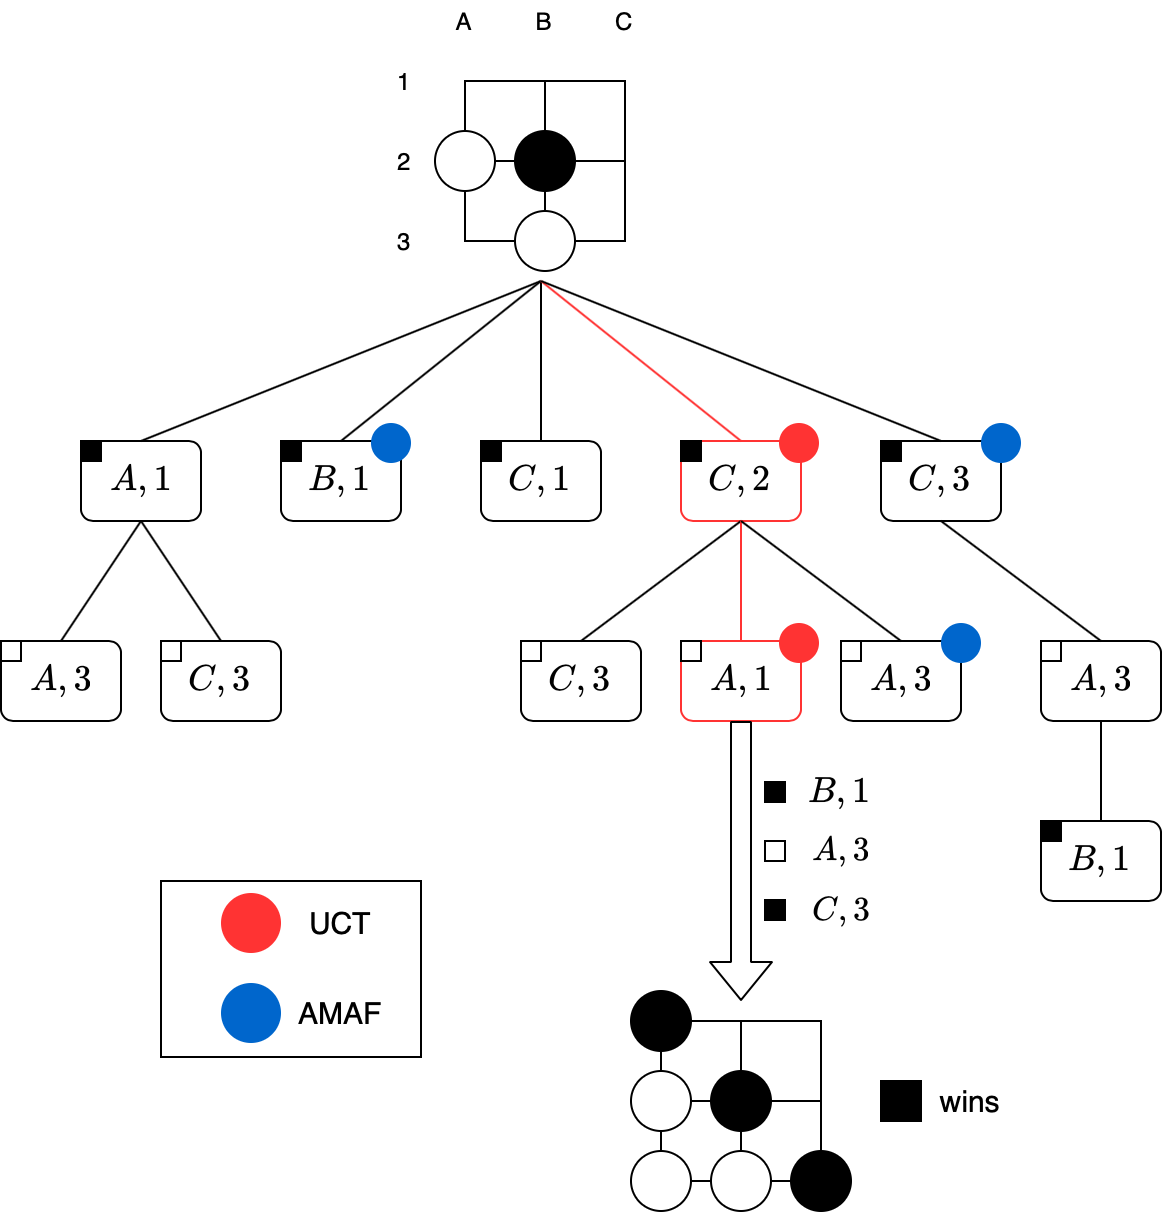
\includegraphics[width=0.65\textwidth]{img/amaf.png}
    \caption{The AMAF-heuristic updates all nodes that are used in the simulation as if they were selected by UCT directly. [modified image from \cite{browne2012survey}]}
    \label{fig:amaf}
\end{figure}
\newpage
\textit{RAVE} is a way of combining the UCT value $Q(\cdot)$ and AMAF score $AMAF(\cdot)$ for an action $a$ at a state $s$ via the equation:
\begin{equation*}
    RAVE(v) = (1-\beta(v)) \cdot Q(v) + \beta(v) \cdot AMAF(v')
\end{equation*}
where 
\begin{equation*}
    \beta(v) = \sqrt{\frac{K}{3 \cdot N(v) + K}}
\end{equation*}
$N(v)$ denotes the number of visits to node $v$. The term $AMAF(v')$ is the average result of all simulations (i.e., the backpropagated value $\Delta$) in which $v$ was selected after $v$ was visited. $v'$ is an ancestor of $v$. Which ancestor is dependent on the actual formulation, in its basic form \textit{RAVE} always selects the direct predecessor of $v'$ on the path through the search tree. \textit{GRAVE}, described below, modifies this selection procedure. $K$ is the so-called \textit{equivalence parameter} which determines the number of simulations where UCT and AMAF are both considered with equal weight. Intuitively, this combination of a node and its predecessors results in generalizing simulation results to the whole subtree of the node.
\paragraph{GRAVE}
RAVE and its generaliztion GRAVE \cite{cazenave2015generalized} are both answers to the following AMAF-tradeoff: Consider a node representing state $s$ at any point in the search tree. If we want to combine its UCT value and the AMAF-value of its predecessors it is not obvious which predecessor we should choose: If we choose the direct predecessor $s'$ (as does RAVE) its AMAF-value is similar to that of $s$ but less accurate overall since the number of times $s'$ was used in a simulation or chosen directly decreases the deeper we traverse the search tree. If we go further up the tree, i.e., choose more distant predecessors, the relationship between $s$ and $s'$ becomes more distant which usually means that the associated AMAF-values are also less close. However, $s'$ is part of simulations more often so all associated values are more precise in general. GRAVE addresses these problems by relying on an additional parameter \textit{ref}. It picks $s'$ as the closest predecessor that has been used at least \textit{ref} times in simulations. It is thus a true generalization as setting \textit{ref} to zero results in RAVE. In experiments with Go GRAVE performs better than either RAVE or UCT.
\paragraph{Parameter Randomization and GGP}
Sironi and Winands \cite{sironi2019comparing} focus on MCTS as a search strategy in \textit{General Game Playing} (GGP), that is the creation of agents that learn to play a variety of games while being given only their rules. These agents usually have only a limited time to prepare and execute their moves. To this end they need good (i.e., fast and accurate) search strategies to predict the course of the game. When MCTS is used in this scenario the actual actions taken by the search are controlled by the user via a number of parameters. Which values of these parameters are optimal depends on the game but since this is unknown in advance parameter tuning is often simply done offline by taking some aggregate of parameters tested on a set of games. An alternative approach is online tuning of parameters, i.e., adapting the MCTS-variant used while actually playing the game. However, since the time available for adjustments is so short randomizing parameters often results in similar performance. It should be noted however that this does not mean just assigning truly random numbers but rather the specific mapping of parameters to a set of possible values depending on the game and the role the agent plays in it. There are four general strategies for randomizing parameters:
\begin{itemize}
    \item \textit{Per run}: Update once before the game is started.
    \item \textit{Per turn}: Update every time the agent has to take a turn.
    \item \textit{Per simulation}: Update every time a new simulation is started (similar to online tuning).
    \item \textit{Per state}: Update every time a state is visited during a simulation.
\end{itemize}
Experimentally they show that tuning the parameters once \textit{per simulation} leads to the best performance.


\subsection{Real-Time}
\label{ss:real_time}
In the context of developing agents to play the arcade game Ms Pac-Man Pepels et al. \cite{pepels2014real} propose a variety of modifications to MCTS that enable real-time search, that is, search within invariable time constraints. To this end they define an array of modifications that are specific to the game in their formulation but can be generalized. Two of them are described below.
\begin{figure}[ht]
    \centering
    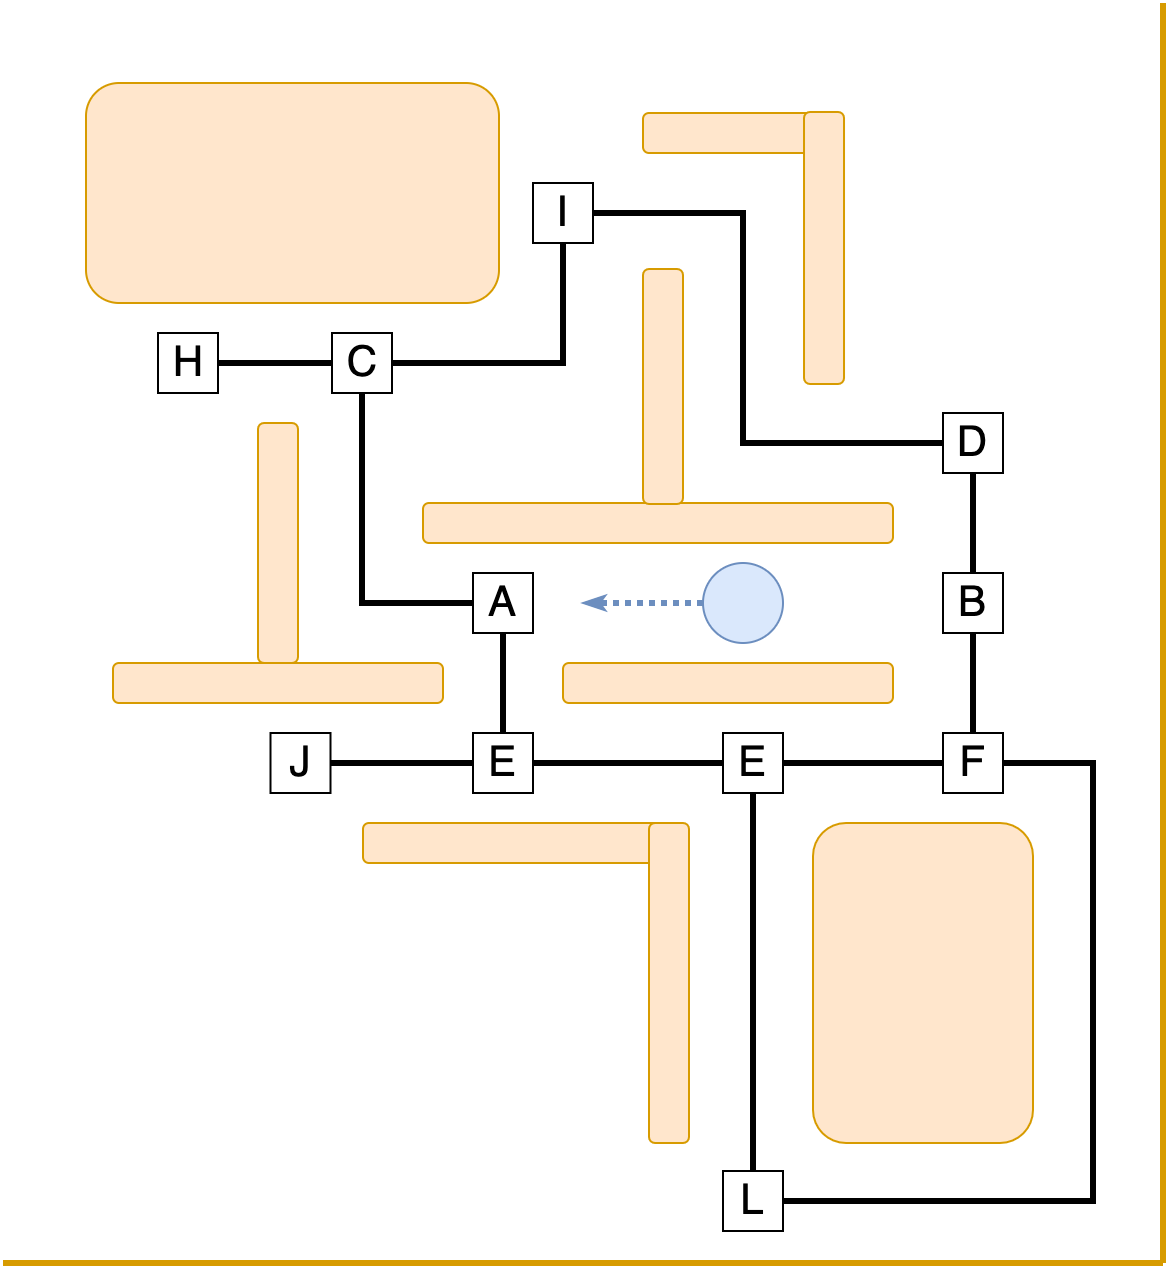
\includegraphics[width=0.5\textwidth]{img/mspacman.png}\\
    \vspace*{0.7cm}
    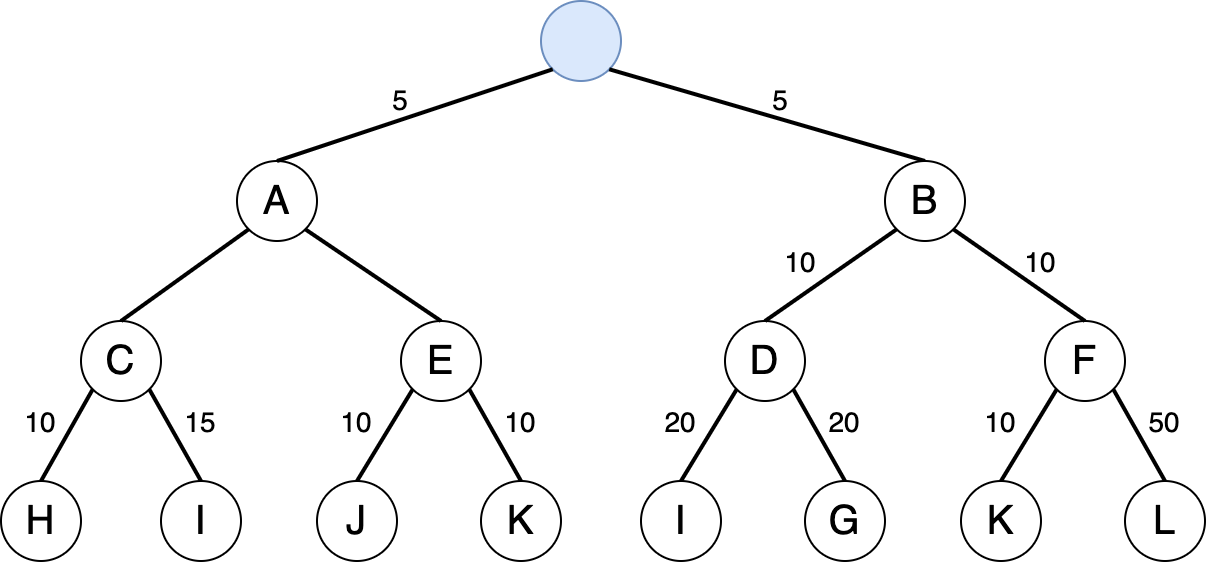
\includegraphics[width=0.6\textwidth]{img/mspacman-tree.png}
    \caption{A sample game state of Ms. Pac-Man and its corresponding search tree. [modified image from \cite{pepels2014real}]}
    \label{fig:mspacman}
\end{figure}
One aspect concerns the creation and use of the search tree. This tree discretizes the complex game state. As shown in figure \ref{fig:mspacman} nodes represent junctions in the game maze. These nodes are connected by edges with an associated length representing the distance that the player has to travel to reach them. Within \enquote{corridors} there are no decisions to be made and moves that lead back to the parent are not considered and modeled. Opponents are not represented as nodes at all. Their movements are simulated while the player traverses the tree and are an additional factor in the game state given by the player's nodes, making these states themselves only approximations. Upon reaching a node (i.e., a junction) the children considered in the expansion step are those that are \begin{enumerate*}[label=\roman*)]
    \item directly reachable (i.e., neighbors of the current junction)
    \item have a distance that would make the length of the search path no longer than a parameter $T_{path}$.
\end{enumerate*} The last requirement limits the depth of the search tree.

The other aspect concerns the reuse of the search tree since the quality of the results of Monte Carlo methods depends on the number of simulations which is necessarily small in real-time scenarios. Additionally, Pac-Man follows a long-term reasoning heuristic (a \textit{plan}). Starting the search over every turn makes such long term reasoning impossible. However, simply keeping an old plan may lead to bad decisions since the values change over time, making the information used outdated. Two techniques are used to mitigate this problem when reusing trees. One is \textit{Rule-Based Reuse}: If one of a set of conditions is met the existing tree is discarded and a new one is built. While the exact conditions are game-specific, the death of the player is a prominent example. The second technique is \textit{Continuous Decay}: The values stored at nodes describing the state of the game are multiplied by a parameter $\gamma \in [0,1]$ at the beginning of each turn. Setting this parameter to zero means no reuse since all values are discarded and setting it to one means no decay at all.


Soemers et al. \cite{soemers2016enhancements} present eight enhancements for real-time MCTS, again in the context of real-time games. Four examples are:
\begin{enumerate}[label=\alph*)]
    \item \textit{Breadth-First Tree Initialization}: Sometimes the number of simulations that can be executed during a turn is smaller than the number of possible actions. This can lead to near-random behavior like selecting an action that leads to a direct loss. This problem is mitigated prior to the start of MCTS by executing a one-step Breadth-First Search from the root node generating all its successors. Then for every successor $M$ simulations are executed and their results backpropagated. Now the actual search is started where there is now information available to avoid bad first moves. One modification is to save the results of the $M$ simulations directly in the successor nodes for reuse later and thereby reduce the overhead.
    \item \textit{Loss Avoidance}: If there are many loss states in a game tree the estimation of a node generated by MCTS can be overly negative. That is, if a node has many children leading to a loss state and only a few leading to a win state simulations will mostly encounter loss nodes and return a low value (for example when crossing rivers in Frogger). \textit{Loss Avoidance} deals with this problem as follows: The first time a node is visited losses are ignored and alternatives are explored immediately. More precisely, any time a simulation involving an unexplored node ends in a loss the result is not backpropagated right away but instead the algorithm backtracks and explores the neighboring nodes. After all alternatives are exhausted only the result of the highest value is backpropagated back to the root.
    \item \textit{Novelty-Based Pruning}: Often there are many redundant paths through the game tree. The aim of \textit{Novelty-Based Pruning} is to prune nodes in such redundant paths. To this end, a novelty measure $nov(s)$ is introduced which assigns each state (node) a score that is high if it is redundant by being very similar to other states in its neighborhood $N(s)$. This set consists of the union of four sets of states, namely 
    \begin{enumerate}[label=\roman*)]
        \item the siblings on the \enquote{left} side of $s$
        \item the parent of $s$, denoted as $p(s)$
        \item the siblings of $p(s)$
        \item the neighborhood of $p(s)$, i.e., $N(p(s))$
    \end{enumerate}
    Note that the first set introduces non-determinism since the states are generally not ordered but still only the left siblings are chosen. Now we can define $nov(s,N(s))$ as the size of the smallest tuple of features that is true in $s$ and not true in $N(s)$. States with a high $nov(\cdot)$ value are pruned and the number of \enquote{unnecessary} paths reduced. This way we do not necessarily avoid bad paths but redundant ones.
    \item \textit{Knowledge-Based Evaluations}: Depending on the game it is often the case that simulations do not find a terminal state or one that changes the score. In such cases the same value is returned for most nodes and no meaningful information is gained. To distinguish between states that have the same evaluation a heuristic function is used. First any object in the game is assigned a type (say, \enquote{wall}, \enquote{enemy}, \enquote{friendly}) and a weight $w_i > 0$ is computed for every type. Let $\Delta_{s_0}$ and $\Delta_{s_T}$ denote the evaluation of the current game state and that of the final state of a simulation. Let $d_0(i)$ and $d_T(i)$ denote the distance to the closest object of type $i$ from the initial state and the terminal state, computed via the $A^\star$ pathfinding algorithm. Now a heuristic value given by the equation $\sum_i w_i \cdot (d_0(i) - d_T(i))$ is added to $\Delta_{s_T}$. Intuitively this heuristic computes the distance to \enquote{interesting} objects of state $s_T$ compared to $s_0$. 
\end{enumerate}
\newpage
\subsection{Multiple Agents}
\label{ss:multi_agents}
\paragraph{Multi-Agent MCTS}
Most MCTS research is focussed on competitive games, i.e., games where two or more players play against each other and each aim to win themselves. Zerbel and Ylinemi \cite{zerbel2019multiagent} focus instead on cooperation between multiple agents. That is games where multiple agents still have individual policies but have to coordinate them to achieve a common goal. The proposed algorithm \textit{Multi-Agent MCTS} (MAMCTS) works in episodes (i.e., discrete turns). First each agent executes the four steps of MCTS Node Selection, Expansion, Simulation and Backpropagation on its own. After that each agent selects the best policy from its own tree and executes the actions contained in this policy. Now, crucially, the agents (or more precisely, their policies) are compared using difference evaluations. Using this calculated difference reward their search trees are updated. Finally the internal state of each agent is reset and the next episode is executed.
\paragraph{Decentralized, Multi-Agent Planning}
In the context of robot move planning Best et al. \cite{best2019dec} propose a variation of MCTS that is both decentralized and online called \textit{Dec-MCTS}. Each robot is part of a joint action space, it optimizes its own planning locally via a probabilistic distribution over all plans and periodically exchanges its search tree with other robots in a compressed version. This information is then used to update its own plans (i.e. the distribution thereof). To this end, they also define a new tree expansion policy called \textit{D-UCT} which is, in turn, a generalization of \textit{D-UCB} \cite{garivier2011upper}.

\begin{figure}[ht]
    \centering
    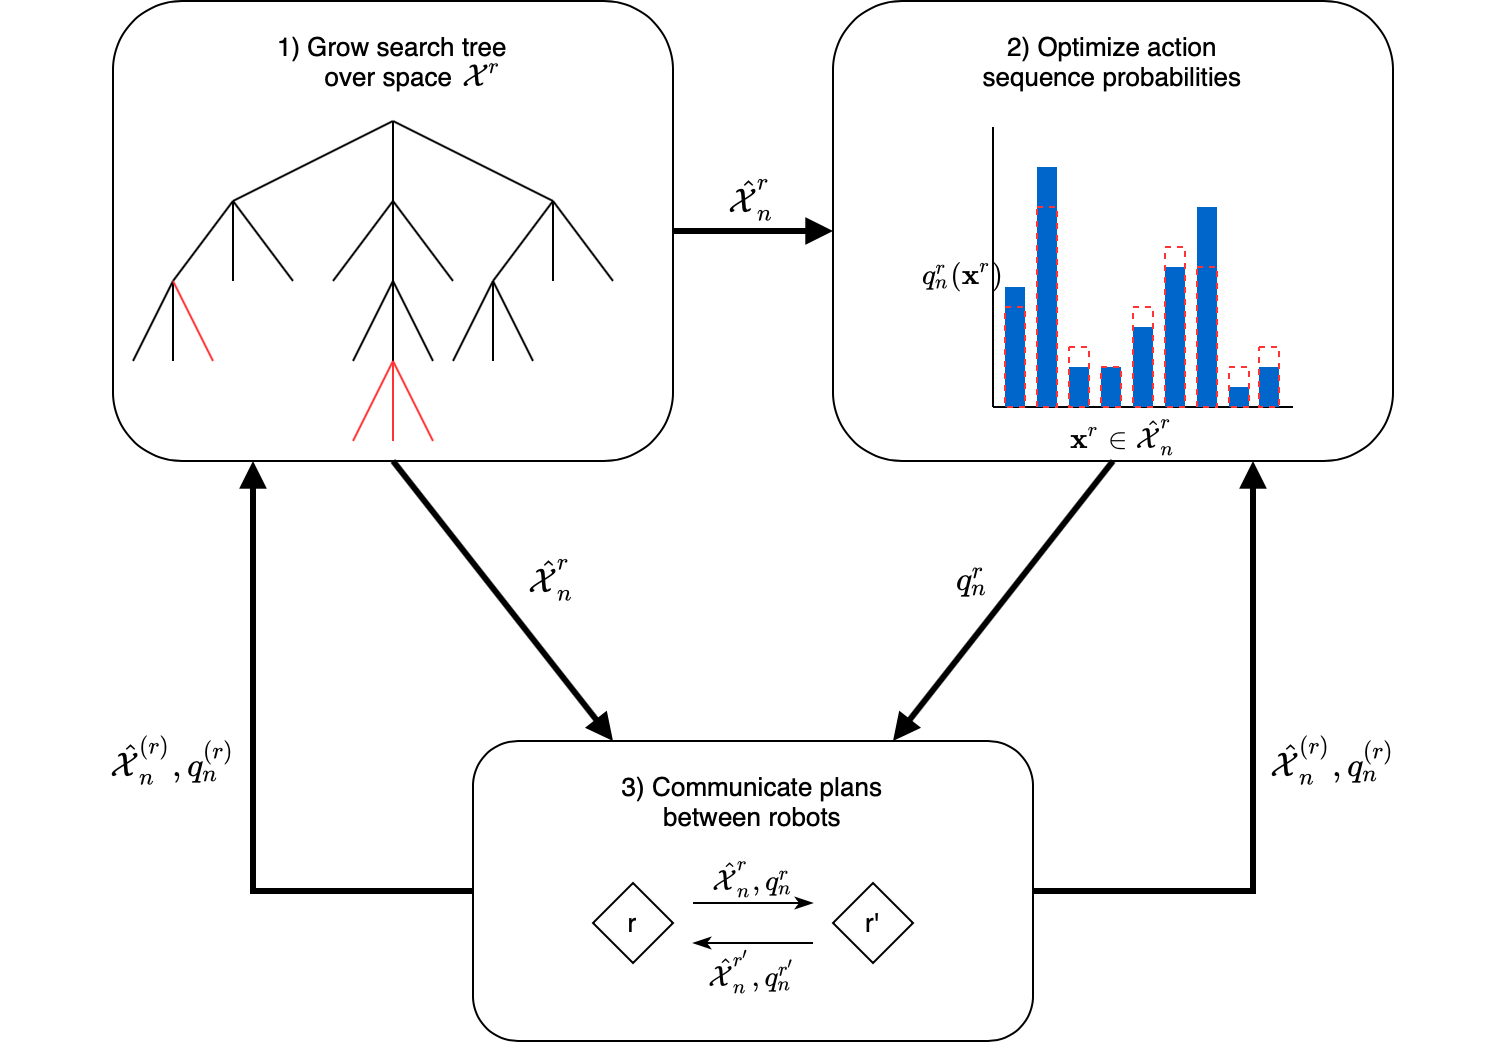
\includegraphics[width=0.9\textwidth]{img/dec-mcts.png}
    \caption{The three basic steps of Dec-MCTS. [modified image from \cite{best2019dec}]}
    \label{fig:dec_mcts}
\end{figure}

The problem to be solved can be stated as follows: Each robot $r$ in the set of robots $\{1,\ldots,R\}$ plans its personal sequence of future actions $ \mathbf{x}^r \coloneqq (x_1^r,x_2^r,\ldots)$. An action $x_j^r$ has a cost $c_j^r$ and the cost of all actions must not exceed the robots budget $B^r$. Let $\mathcal{X}^r$ denote the set of all possible action sequences $\mathbf{x}^r$ for a robot r and let $\mathbf{x} \coloneqq \{\mathbf{x}
^1, \ldots , \mathbf{x}^R\}$ denote this set for all robots. 
Now the aim is to maximize a global objective function $g(\mathbf{x})$. This function is known to each robot but not the action sequences selected by the others. This information must be exchanged in an asynchronous manner which usually is additionally restricted in other ways (e.g. limits on size, number and timing of messages). 
The proposed Algorithm Dec-MCTS is displayed in Figure \ref{fig:dec_mcts}. It consists of three phases and is running asynchronously on all robots until the computational budget is exhausted. In particular the algorithm is fault tolerant with respect to the success of the communication with other robots. 

Consider robot $r$ running the $n$-th iteration of the algorithm. Its current plan is defined as a probability distribution $q^r_n$ over all action sequences $\mathcal{X}^r$. To make the problem tractable the actual domain is refined to $\Hat{\mathcal{X}}^r_n \subset \mathcal{X}^r$. That is the subset of all action sequences where the probability is greater than zero. The search tree $\mathcal{T}^r$ contains only the actions of robot $r$, each edge representing one action and paths representing valid action sequences. In the first phase this tree is grown while considering the (set of) plans of the other robots $q_n^{(r)}$ over $\Hat{\mathcal{X}}_n^{(r)}$ using the algorithm discussed below. In phase two (executed periodically) the domain and action sequences are optimized using a decentralized adaptation of gradient descent. Afterwards these changes are communicated to the other robots in phase three.

We now focus on step one: Both the tree and default policies of the standard MCTS-algorithm are adapted. To define the tree policy a so-called \textit{discounted version} of UCT is introduced. Given a parameter $\gamma \in [0,1]$ the definitions of $N(\cdot)$, $Q(\cdot)$ and UCT are modified:
\begin{equation*}
    N_\gamma(s) \coloneqq \sum_{u = 1}^t \gamma^{t-u} \cdot \mathbb{I}_t(s)
\end{equation*}
The function $\mathbb{I}_t(s)$ is equal to one if $s$ has been selected at turn $t$ and zero otherwise.
\begin{equation*}
    \Bar{Q}_\gamma(s) \coloneqq \frac{1}{N_\gamma(s)}\sum_{u = 1}^t  \gamma^{t-u} \cdot Q^u(s) \cdot \mathbb{I}_u(s)
\end{equation*}
Now the child selection function is given via:
\begin{equation*}
    \text{D-UCT}(\gamma,s) =  \Bar{Q}_\gamma(s) + C_p \cdot \sqrt{\frac{2 \ln N_\gamma(s)}{N_\gamma(s')}}
\end{equation*}
The default policy used for simulations is changed as follows. The reward predicted by a simulation can be seen as an approximation for $\mathbb{E}[g]$. Since $g$ is a function of all plans we first need a sample of the other robots' plans $q_n^{(r)}$ before the simulation starts. However, since this sample may be inaccurate (especially compared to our own plans $q_n^{(r)}$) we execute the simulation now with respect to $g$ but to a local utility function $f
^r$ that is less sensitive to the possible high variance of $q_n^{(r)}$. Now the simulation is executed and the results are backpropagated.   
\subsection{Evolutionary Algorithms}
\label{ss:evo_alg}
Lucas et al. \cite{lucas2014fast} describe a way of incorporating an evolutionary algorithms into  MCTS in place of a heuristic. Multiple variations (\enquote{individuals}) of the same MCTS-algorithm with different parameters are instantiated. Then their performance (their \enquote{fitness}) is evaluated using a metric and only the best ones get to \enquote{reproduce} and/or are modified using \enquote{mutations}. There are two general ways of evaluating fitness: Either the fitness of the algorithm is evaluated over a set of games and the actual effects of the algorithm (or MCTS-\textit{agent}) are viewed as a black box whose parameters can be tuned. Or, and this is the approach taken here, the evaluation happens during the simulation (i.e., step 3 in the description given above). Each individual is defined via a parameter-vector and is evaluated \begin{enumerate*}[label=\alph*)]
    \item on the same tree
    \item every time the default policy is executed 
\end{enumerate*}. Consequently, there is much more information available and the evolution can happen faster. The executed steps are displayed in Algorithm \ref{alg:fastevo_mcts}. At first a parameter vector $w$ is drawn and a new statistics-object $S$ is initialized. Now the tree and default policies controlled by $w$ are sampled $K$ times and the resulting metrics (such as min/max, average reward) are used to evaluate the fitness of the parameter vector. After the budget (time or computational resources) is used up the best vector is chosen and returned.
\begin{algorithm}[ht]
\begin{algorithmic}
\Function{FastEvoMCTS}{$K, v_0$} 
    \While{within computational budget}
    \State $w \gets$ \Call{evo.getNext}{\null}
    \State Initialize $S$
    \For{$i \coloneqq 1$ to $K$}
    \State $v_l \gets$ \Call{TreePolicy}{$v_0,T(w)$}
    \State $\Delta \gets$ \Call{DefaultPolicy}{$s(v_l),D(w)$}
    \State \Call{Backup}{$S,\Delta$}
    \State \Call{UpdateStats}{$S,\Delta$}
    \EndFor
    \State \Call{evo.setFitness}{$\mathbf{w},S$}
    \EndWhile
    \State $\mathbf{w} \gets$ \Call{evo.getBest}{\null}
    \State $a \gets$ \Call{recommend}{$v_0$}
    \State \Return $(w,a)$
\EndFunction
\end{algorithmic}
\caption{Fast Evolutionary MCTS.}
\label{alg:fastevo_mcts}
\end{algorithm}

Benbassat and Supper \cite{benbassat2014evomcts} present another evolutionary approach to MCTS that focuses on zero-sum, deterministic, full-knowledge board games while remaining scalable.